\documentclass[systemskiss/skiss.tex]{subfiles}

\begin{document}
\section{Kommunikationsmodul}
Kommunikationsmodulen är den modul som ska kommunicera med de andra modulerna samt ha en trådlös koppling till den bärbara datorn. 
\subsection{Översiktlig beskrivning av modulen}
\begin{figure}[h]
    \centering
    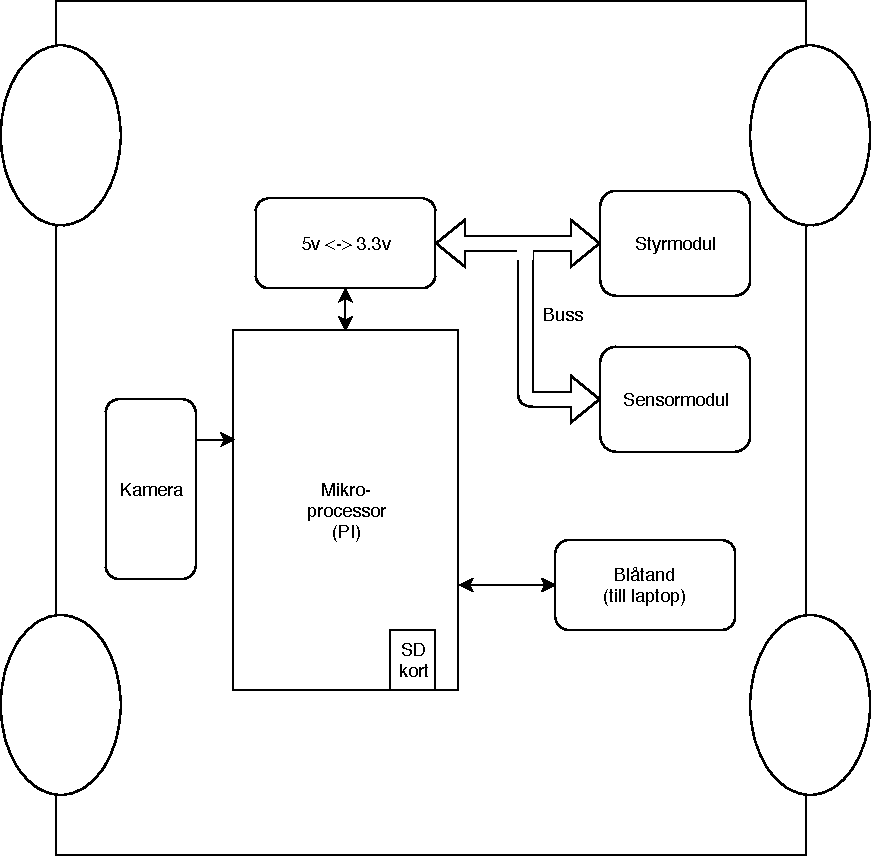
\includegraphics[width=0.6\linewidth]{systemskiss/figures/kommodul.pdf}
    \caption{Övergripande bild över komunikationsmodulen}
    \label{fig:komskiss}
\end{figure}
Processorn i modulen kommer vara en Rasberry Pi 3. Den är kraftfull och utrustad med en rad verktyg som modulen kan ha användning för. Bland annat att kunna montera kameran som systemet ska använda för navigering via bildbehandling. Den har också tillräckligt stort minne som kan användas till att förvara kartan m.m. Processorn har även stöd för att koppla in trådlösa enheter, vilket gör att den bärbara datorn lätt kan anslutas. Modulen ska vara kopplad via någon typ av databuss till både styr- och sensormodulen. För att den kopplingen  ska vara möjlig behövs ett filter eller en transformator som gör om övriga systemets 5 volt spänningar till processorns 3.3 volt pinnar. En enkel skiss av modulen finns i figur \ref{fig:komskiss}.
\end{document}

